\documentclass[aspectratio=169]{beamer}
\usepackage{amsmath}
\usepackage{amssymb}
\usepackage{tikz}
\usepackage{wasysym}
\usepackage{tikzsymbols}
\usepackage{xcolor}
\usepackage{animate}     % Option 1: play a PNG frame sequence
\usepackage{multimedia}  % Option 2: embed a video file (needs -shell-escape)
\usetikzlibrary{shapes,backgrounds,patterns}

% --- added for these slides -------------------------------------------------
\usepackage{pgfplots}
\pgfplotsset{compat=1.18, legend cell align=left}
\usetikzlibrary{arrows.meta,decorations.pathreplacing,calc,positioning}
\usepackage{listings}
\usepackage{booktabs}
\usepackage{array}
% ----------------------------------------------------------------------------

% royalblue isn't a base xcolor name, so define it first (this is the default accent)
\definecolor{royalblue}{RGB}{65,105,225}

% ============================================================
%  ACCENT COLOR: change ONE line below to switch the theme
%  Choose one of: royalblue , red , black
% ============================================================
\colorlet{accent}{royalblue}
% \colorlet{accent}{red}
% \colorlet{accent}{black}
% ============================================================

% Use default theme with white background
\usetheme{default}

% Make everything white/black, with the chosen accent color for structure
\setbeamercolor{background canvas}{bg=white}
\setbeamercolor{normal text}{fg=black}
\setbeamercolor{structure}{fg=accent}
\setbeamercolor{frametitle}{fg=accent,bg=white}
\setbeamercolor{title}{fg=accent}
\setbeamercolor{section in toc}{fg=black}
\setbeamercolor{block title}{fg=black,bg=gray!10}
\setbeamercolor{block body}{fg=black,bg=gray!5}
\setbeamercolor{block title example}{fg=black,bg=green!10}
\setbeamercolor{block body example}{fg=black,bg=green!5}
\setbeamercolor{block title alerted}{fg=black,bg=red!10}
\setbeamercolor{block body alerted}{fg=black,bg=red!5}

\usepackage{scalerel}

\newcommand{\subsmall}[1]{_{\scaleto{#1}{4pt}}}
\newcommand{\supsmall}[1]{^{\scaleto{#1}{2pt}}}

% Remove navigation symbols
\setbeamertemplate{navigation symbols}{}

% Simple footline with page numbers (single definition)
\setbeamertemplate{footline}{
    \hfill\makebox[5pt]{%
        \scriptsize\insertframenumber}
    \hspace*{2em}
    \vspace{0.5cm}
}

% Custom command for colored boxes
\newcommand{\cbox}[2]{\colorbox{#1}{\ensuremath{\displaystyle #2}}}

% --- code listings (Python), coloured with the accent -----------------------
\lstdefinestyle{py}{
  language=Python,
  basicstyle=\ttfamily\footnotesize,
  keywordstyle=\color{accent}\bfseries,
  commentstyle=\color{gray}\itshape,
  stringstyle=\color{green!45!black},
  showstringspaces=false,
  columns=fullflexible,
  keepspaces=true,
  backgroundcolor=\color{gray!6},
  frame=single, rulecolor=\color{gray!30},
  xleftmargin=2pt, xrightmargin=2pt,
  escapeinside={(*}{*)}
}
\lstset{style=py}

% --- shared plot style for the three "bound" pictures ------------------------
\pgfplotsset{
  boundplot/.style={
    width=5.9cm, height=4.6cm,
    axis lines=left, xmin=0, xmax=10, ymin=0, ymax=12,
    xtick=\empty, ytick=\empty,
    xlabel={$n$}, ylabel={time},
    every axis x label/.style={at={(axis description cs:1,0)},anchor=north east},
    every axis y label/.style={at={(axis description cs:0,1)},anchor=south east},
    samples=160, thick, clip mode=individual
  }
}

\title{Limits \& Convergence of Algorithms}
\subtitle{Growth rates revisited, sequences, and the order of convergence}
\author{Sharareh Sayyad}
\institute{Washington state University}
\date{September 30, 2026}

\begin{document}

\frame{\titlepage}

\begin{frame}{Outline}
\tableofcontents
\end{frame}

% ============================================================
\section{Review: polynomial vs.\ exponential growth}
% ============================================================

\begin{frame}{Review: polynomial vs.\ exponential growth}
\begin{columns}[T]
\begin{column}{0.48\textwidth}
\begin{block}{Polynomial: $O(n^a)$}
\small
\begin{itemize}
  \item nested loops: $n$, $n^2$, $n^3$, \ldots
  \item \textbf{double} $n$ $\Rightarrow$ work $\times\,2^a$
\end{itemize}
\end{block}
\begin{block}{Exponential: $O(b^{\,n})$, \ $b > 1$}
\small
\begin{itemize}
  \item try every subset: $2^n$
  \item \textbf{add one} to $n$ $\Rightarrow$ work $\times\,b$
\end{itemize}
\end{block}
\end{column}
\begin{column}{0.48\textwidth}
\centering
\small
\renewcommand{\arraystretch}{1.15}
\begin{tabular}{rrr}
\toprule
$n$ & $n^3$ & $2^n$ \\
\midrule
$10$ & $1\,000$ & $1\,024$ \\
$20$ & $8\,000$ & $1.0\times10^{6}$ \\
$40$ & $64\,000$ & $1.1\times10^{12}$ \\
$80$ & $512\,000$ & $1.2\times10^{24}$ \\
\bottomrule
\end{tabular}\\[8pt]
\begin{exampleblock}{Already a limit!}
\footnotesize For any $a$ and any $b > 1$:
\ $\displaystyle\lim_{n\to\infty} \frac{n^a}{b^{\,n}} = 0$.\\
Every exponential eventually beats every polynomial.
\end{exampleblock}
\end{column}
\end{columns}
\end{frame}

\begin{frame}{Which axes make it a straight line?}
\centering
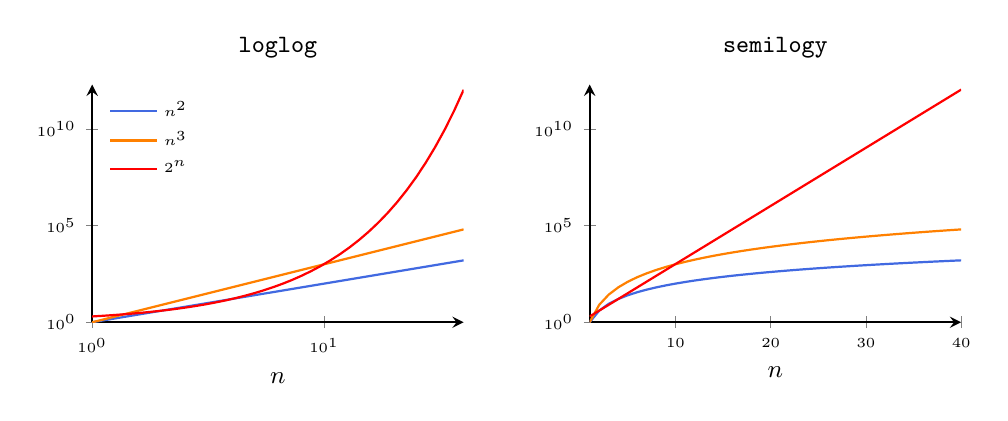
\begin{tikzpicture}
\begin{axis}[name=ll, width=6.3cm, height=4.6cm, xmode=log, ymode=log, axis lines=left,
  xmin=1, xmax=40, ymin=1, ymax=2e12, xlabel={$n$}, title={\small \texttt{loglog}}, thick,
  tick label style={font=\tiny}, label style={font=\small},
  legend style={font=\tiny, draw=none, at={(0.02,0.98)}, anchor=north west}]
  \addplot[accent, domain=1:40, samples=40] {x^2}; \addlegendentry{$n^2$}
  \addplot[orange, domain=1:40, samples=40] {x^3}; \addlegendentry{$n^3$}
  \addplot[red, domain=1:40, samples=40] {2^x}; \addlegendentry{$2^n$}
\end{axis}
\begin{axis}[at={($(ll.east)+(1.6cm,0)$)}, anchor=west, width=6.3cm, height=4.6cm, ymode=log, axis lines=left,
  xmin=1, xmax=40, ymin=1, ymax=2e12, xlabel={$n$}, title={\small \texttt{semilogy}}, thick,
  tick label style={font=\tiny}, label style={font=\small}]
  \addplot[accent, domain=1:40, samples=40] {x^2};
  \addplot[orange, domain=1:40, samples=40] {x^3};
  \addplot[red, domain=1:40, samples=40] {2^x};
\end{axis}
\end{tikzpicture}\\[4pt]
\small
\renewcommand{\arraystretch}{1.15}
\begin{tabular}{llll}
\toprule
growth & take logs & straight on & slope \\
\midrule
$t \approx c\,n^a$ & $\log t \approx a\log n + \log c$ & \texttt{loglog} & $a$ \ (exponent) \\
$t \approx c\,b^{\,n}$ & $\log t \approx n\log b + \log c$ & \texttt{semilogy} & $\log b$ \ ($b = e^{\text{slope}}$) \\
\bottomrule
\end{tabular}
\end{frame}

\begin{frame}[fragile]{Recipe: fit the slope, then test the model}
\begin{columns}[T]
\begin{column}{0.44\textwidth}
\begin{lstlisting}[basicstyle=\ttfamily\scriptsize]
# polynomial model: slope = a
a = np.polyfit(np.log(ns),
               np.log(ts), 1)[0]

# exponential model: slope = log b
s = np.polyfit(ns, np.log(ts), 1)[0]
b = np.exp(s)
\end{lstlisting}
\small
\texttt{polyfit} \textbf{always} returns a number, even for the wrong model. So how do we know which model is right?
\vspace{6pt}

\scriptsize Reminder: fit only the large-$n$ part, as last time.
\end{column}
\begin{column}{0.53\textwidth}
\begin{exampleblock}{The split test}
\small Fit the model twice: on the \textbf{first half} of the data, then on the \textbf{second half}. Right model: both fits \textbf{agree}. Wrong model: the value \textbf{drifts}.
\end{exampleblock}
\footnotesize \textbf{Example.} Data $t = n^3$, for $n = 10, 12, \ldots, 40$:\\[3pt]
\centering
\renewcommand{\arraystretch}{1.15}
\scriptsize
\begin{tabular}{lccc}
\toprule
model & \shortstack{first half\\$n = 10\ldots24$} & \shortstack{second half\\$n = 26\ldots40$} & verdict \\
\midrule
polynomial, $a$ & $3.00$ & $3.00$ & \textcolor{green!50!black}{\textbf{same}} \\
exponential, $b$ & $1.20$ & $1.10$ & \textcolor{red}{\textbf{drifts}} \\
\bottomrule
\end{tabular}\\[3pt]
\raggedright \footnotesize So the data is polynomial, $O(n^3)$, not exponential.
\end{column}
\end{columns}
\end{frame}

% ============================================================
\section{Limits of sequences}
% ============================================================

\begin{frame}{Sequences and limits}
\begin{columns}[T]
\begin{column}{0.52\textwidth}
\small
A \textbf{sequence} is a list of numbers $x_0, x_1, x_2, \ldots$ indexed by $k$.
\begin{block}{Definition}
$x_k \to x_\ast$ (``converges to $x_\ast$'') if for every tolerance $\tau > 0$ there is a $K$ with
\[ |x_k - x_\ast| < \tau \quad \text{for all } k \ge K. \]
\end{block}
\footnotesize \textbf{In words:} choose any tolerance $\tau$, however small. After some index $K$, \textbf{every} term stays within $\tau$ of $x_\ast$.
\begin{exampleblock}{Example: $x_k = 1/k \to 0$}
\footnotesize Tolerance $\tau = 0.01$: take $K = 101$. Every $k \ge 101$ gives $1/k < 0.01$.\\
Smaller $\tau$ just needs a larger $K$.
\end{exampleblock}
\end{column}
\begin{column}{0.45\textwidth}
\small
\renewcommand{\arraystretch}{1.25}
\begin{tabular}{ll}
\toprule
sequence & behaviour \\
\midrule
$1/k$ & $\to 0$ \\
$(1+1/k)^k$ & $\to e$ \\
$\sum_{j=1}^{k} 1/j^2$ & $\to \pi^2/6$ \\
$(-1)^k$ & no limit (oscillates) \\
$k^2$ & $\to \infty$ (diverges) \\
\bottomrule
\end{tabular}\\[8pt]
\footnotesize Converging means the terms settle down to \textbf{one} finite number.
\end{column}
\end{columns}
\end{frame}

% ============================================================
\section{Algorithms as sequences}
% ============================================================

\begin{frame}{An algorithm's output is a sequence}
\begin{columns}[T]
\begin{column}{0.5\textwidth}
\small
Record the output after every iteration:
\[
x_0 \xrightarrow{\ g\ } x_1 \xrightarrow{\ g\ } x_2 \xrightarrow{\ g\ } \cdots, \qquad x_{k+1} = g(x_k).
\]
\renewcommand{\arraystretch}{1.2}
\footnotesize
\begin{tabular}{ll}
\toprule
algorithm & $x_k$ \\
\midrule
Newton for $\sqrt2$ & $x_{k+1} = \tfrac12(x_k + 2/x_k)$ \\
$\cos$ iteration & $x_{k+1} = \cos x_k$ \\
partial sums of a series & $S_{k+1} = S_k + a_{k+1}$ \\
\bottomrule
\end{tabular}
\end{column}
\begin{column}{0.47\textwidth}
\begin{block}{Where does it converge?}
\small If $x_k \to x_\ast$ and $g$ is continuous, take the limit on both sides of $x_{k+1} = g(x_k)$:
\[ x_\ast = g(x_\ast). \]
The limit must be a \textbf{fixed point} of $g$.
\end{block}
\footnotesize So: \textbf{solve $x = g(x)$ to find the candidates}, then ask which one (if any) the iteration actually reaches.\\[4pt]
Newton: $x = \tfrac12(x + 2/x) \iff x^2 = 2$.
\end{column}
\end{columns}
\end{frame}

\begin{frame}[fragile]{Seeing it: the cobweb plot}
\begin{columns}[T]
\begin{column}{0.52\textwidth}
\footnotesize
\textbf{Why draw it?} The numbers $x_0, x_1, \ldots$ tell you \emph{whether} the iteration settles; the cobweb shows \emph{where} (where $y = g(x)$ crosses $y = x$) and \emph{how} (spirals in, walks in, or runs away).\\[3pt]
\textbf{How:} each iteration draws \textbf{two} line segments:
\begin{enumerate}\setlength{\itemsep}{0pt}
  \item \textbf{vertical} to the curve: $(x_k, x_k) \to (x_k, x_{k+1})$;
  \item \textbf{horizontal} back to $y = x$: $(x_k, x_{k+1}) \to (x_{k+1}, x_{k+1})$.
\end{enumerate}
\begin{lstlisting}[basicstyle=\ttfamily\scriptsize]
x = np.linspace(0, 1.1, 200)
plt.plot(x, np.cos(x))    # curve y = g(x)
plt.plot(x, x, "k")       # line  y = x
xk = 0.2                  # start x_0
for k in range(10):
    xnew = np.cos(xk)     # x_{k+1} = g(x_k)
    plt.plot([xk, xk], [xk, xnew], "r")
    plt.plot([xk, xnew], [xnew, xnew], "r")
    xk = xnew
\end{lstlisting}
\end{column}
\begin{column}{0.45\textwidth}
\centering
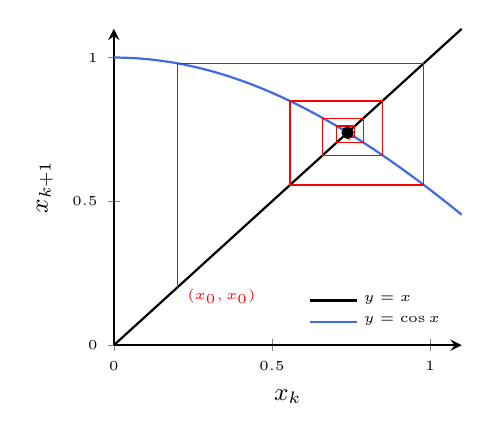
\begin{tikzpicture}
\begin{axis}[width=6cm, height=5.6cm, axis lines=left, xmin=0, xmax=1.1, ymin=0, ymax=1.1,
  xlabel={$x_k$}, ylabel={$x_{k+1}$}, thick, tick label style={font=\tiny}, label style={font=\small},
  legend style={font=\tiny, draw=none, at={(0.98,0.02)}, anchor=south east}]
  \addplot[black, domain=0:1.1, samples=2] {x}; \addlegendentry{$y = x$}
  \addplot[accent, domain=0:1.1, samples=80] {cos(deg(x))}; \addlegendentry{$y = \cos x$}
  \addplot[red, thin, -{Stealth[length=3pt]}] coordinates {(0.2000,0.2000) (0.2000,0.9801) (0.9801,0.9801) (0.9801,0.5570) (0.5570,0.5570) (0.5570,0.8489) (0.8489,0.8489) (0.8489,0.6608) (0.6608,0.6608) (0.6608,0.7895) (0.7895,0.7895) (0.7895,0.7042) (0.7042,0.7042) (0.7042,0.7621) (0.7621,0.7621) (0.7621,0.7234) (0.7234,0.7234)};
  \addplot[only marks, mark=*, mark size=1.8pt, black] coordinates {(0.7391,0.7391)};
  \node[font=\tiny, red, right] at (axis cs:0.2,0.17) {$(x_0, x_0)$};
\end{axis}
\end{tikzpicture}\\[2pt]
\footnotesize $x_{k+1} = \cos x_k$ from $x_0 = 0.2$ spirals in to the crossing $x_\ast \approx 0.739$.
\end{column}
\end{columns}
\end{frame}

\begin{frame}{Which fixed point does the iteration find?}
\begin{columns}[T]
\begin{column}{0.47\textwidth}
\begin{block}{The problem}
\small $g$ can have \textbf{several} fixed points, but the iteration can end at \textbf{at most one}, or at none. Which one, and why?
\end{block}
\begin{exampleblock}{Example: $g(x) = x^2$}
\small Fixed points solve $g(x_\ast) = x_\ast$: \ $x_\ast^2 = x_\ast$, so $x_\ast = 0$ or $x_\ast = 1$.\\[3pt]
\footnotesize
\begin{tabular}{ll}
$x_0 = 0.9$: & $0.81,\ 0.66,\ 0.43,\ \ldots \to 0$ \\
$x_0 = 1.1$: & $1.21,\ 1.46,\ 2.14,\ \ldots \to \infty$
\end{tabular}\\[3pt]
Starting close to $1$ does not help: the iterates move \textbf{away} from $1$.\\[2pt]
Slopes: $g'(x) = 2x$, so $g'(0) = 0$ and $g'(1) = 2$.
\end{exampleblock}
\end{column}
\begin{column}{0.5\textwidth}
\small
\textbf{The reason: the slope of $g$ at $x_\ast$.} Near $x_\ast$, one step multiplies the error by about $g'(x_\ast)$:
\[
x_{k+1} - x_\ast = g(x_k) - g(x_\ast) \approx g'(x_\ast)\,(x_k - x_\ast).
\]
\begin{block}{Local test}
\begin{itemize}
  \item $|g'(x_\ast)| < 1$: error shrinks, $x_\ast$ \textbf{attracts}, with rate $C = |g'(x_\ast)|$;
  \item $|g'(x_\ast)| > 1$: error grows, $x_\ast$ \textbf{repels}.
\end{itemize}
\end{block}
\footnotesize $g(x) = x^2$: \ $0$ attracts, $1$ repels.\\[2pt]
$g(x) = \cos x$, $g'(x) = -\sin x$: at $x_\ast \approx 0.739$, $|g'(x_\ast)| = \sin(0.739) \approx 0.67 < 1$: attracts, error $\times\,0.67$ per step.
\end{column}
\end{columns}
\end{frame}

% ============================================================
\section{Order of convergence}
% ============================================================

\begin{frame}{Order of convergence}
\small
Error $\epsilon_k = |x_k - x_\ast|$. \ The key question: \textbf{how does one iteration shrink the error?}
\begin{block}{Definition}
The convergence has \textbf{order} $q \ge 1$ and \textbf{rate constant} $C$ if
\[ \lim_{k\to\infty} \frac{\epsilon_{k+1}}{\epsilon_k^{\,q}} = C, \qquad 0 < C < \infty . \]
\footnotesize For $q = 1$: \ $C < 1$ is \textbf{linear}, \ $C = 1$ is \textbf{sublinear}.
\end{block}
\vspace{2pt}
\begin{center}
\small
\renewcommand{\arraystretch}{1.25}
\begin{tabular}{p{2.2cm}p{7.2cm}}
\toprule
name & ratio $\epsilon_{k+1}/\epsilon_k$ \\
\midrule
sublinear & \textbf{not} constant: it creeps up to $1$ \newline e.g.\ $\epsilon_k = 1/k$: \ $\tfrac12,\ \tfrac23,\ \tfrac34,\ \ldots \to 1$ \\
linear & constant $C < 1$ \\
superlinear & goes to $0$: each step helps more than the last \\
\bottomrule
\end{tabular}
\end{center}
\end{frame}

\begin{frame}{Sublinear, linear, superlinear on a \texttt{semilogy} plot}
\begin{columns}[c]
\begin{column}{0.46\textwidth}
\renewcommand{\arraystretch}{1.3}
\footnotesize
\begin{tabular}{p{1.7cm}p{4.0cm}}
\toprule
type & on \texttt{semilogy} \\
\midrule
\textcolor{orange}{\textbf{sublinear}} & \textbf{flattens out}: each step gains less \\
\textcolor{accent}{\textbf{linear}} & \textbf{straight line}, slope $\log C$ \\
\textcolor{red}{\textbf{superlinear}} & \textbf{bends down}: each step gains more \\
\bottomrule
\end{tabular}
\end{column}
\begin{column}{0.52\textwidth}
\centering
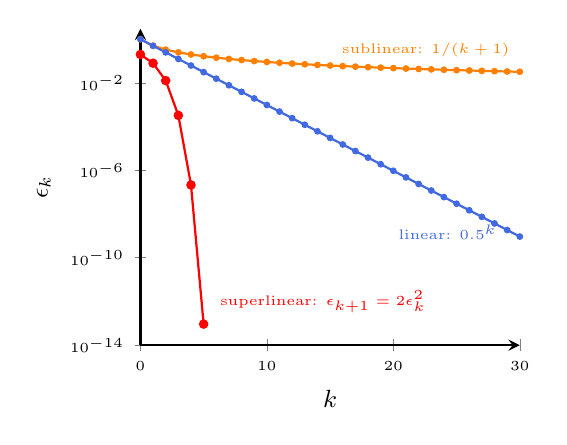
\begin{tikzpicture}
\begin{axis}[width=6.4cm, height=5.6cm, ymode=log, axis lines=left,
  xmin=0, xmax=30, ymin=1e-14, ymax=3, xlabel={$k$}, ylabel={$\epsilon_k$}, thick,
  tick label style={font=\tiny}, label style={font=\small}]
  \addplot[orange, mark=*, mark size=0.8pt] coordinates {(0,1) (1,0.5) (2,0.3333) (3,0.25) (4,0.2) (5,0.1667) (6,0.1429) (7,0.125) (8,0.1111) (9,0.1) (10,0.09091) (11,0.08333) (12,0.07692) (13,0.07143) (14,0.06667) (15,0.0625) (16,0.05882) (17,0.05556) (18,0.05263) (19,0.05) (20,0.04762) (21,0.04545) (22,0.04348) (23,0.04167) (24,0.04) (25,0.03846) (26,0.03704) (27,0.03571) (28,0.03448) (29,0.03333) (30,0.03226)};
  \addplot[accent, mark=*, mark size=0.8pt] coordinates {(0,1) (1,0.5) (2,0.25) (3,0.125) (4,0.0625) (5,0.03125) (6,0.01562) (7,0.007812) (8,0.003906) (9,0.001953) (10,0.0009766) (11,0.0004883) (12,0.0002441) (13,0.0001221) (14,6.104e-05) (15,3.052e-05) (16,1.526e-05) (17,7.629e-06) (18,3.815e-06) (19,1.907e-06) (20,9.537e-07) (21,4.768e-07) (22,2.384e-07) (23,1.192e-07) (24,5.96e-08) (25,2.98e-08) (26,1.49e-08) (27,7.451e-09) (28,3.725e-09) (29,1.863e-09) (30,9.313e-10)};
  \addplot[red, mark=*, mark size=1.3pt] coordinates {(0,0.2) (1,0.08) (2,0.0128) (3,0.0003277) (4,2.147e-07) (5,9.223e-14)};
  \node[orange, font=\tiny, above left] at (axis cs:30,0.05) {sublinear: $1/(k+1)$};
  \node[accent, font=\tiny, below left] at (axis cs:29,1e-8) {linear: $0.5^k$};
  \node[red, font=\tiny, right] at (axis cs:5.5,1e-12) {superlinear: $\epsilon_{k+1} = 2\epsilon_k^2$};
\end{axis}
\end{tikzpicture}
\end{column}
\end{columns}
\end{frame}

\begin{frame}{Measuring $q$: plot $\epsilon_{k+1}$ against $\epsilon_k$}
\begin{columns}[c]
\begin{column}{0.44\textwidth}
\small
Take logs of $\epsilon_{k+1} \approx C\,\epsilon_k^{\,q}$:
\[
\log \epsilon_{k+1} \approx q\,\log \epsilon_k + \log C .
\]
A \textbf{power law} again, so on \texttt{loglog} axes the points $(\epsilon_k, \epsilon_{k+1})$ lie on a line with \textbf{slope $q$}.
\vspace{4pt}
\begin{itemize}\footnotesize
  \item \textcolor{orange}{\textbf{sublinear}}: slope $1$, hugging $y = x$ ($C = 1$: almost no progress);
  \item \textcolor{accent}{\textbf{linear}}: slope $1$, parallel \textbf{below} $y = x$ (by the factor $C = 0.5$);
  \item \textcolor{red}{\textbf{superlinear}}: \textbf{steeper}, here slope $2$.
\end{itemize}
\end{column}
\begin{column}{0.54\textwidth}
\centering
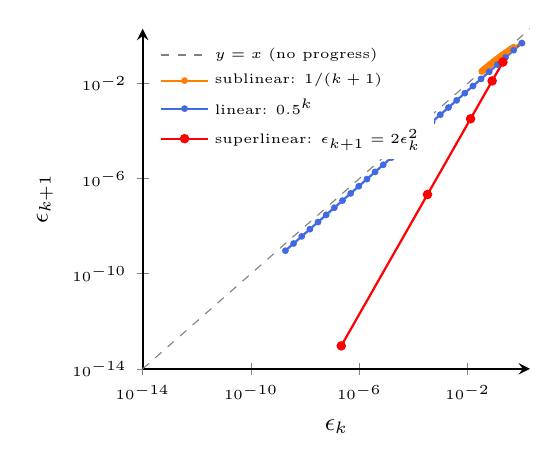
\begin{tikzpicture}
\begin{axis}[width=6.5cm, height=5.9cm, xmode=log, ymode=log, axis lines=left,
  xmin=1e-14, xmax=2, ymin=1e-14, ymax=2, xlabel={$\epsilon_k$}, ylabel={$\epsilon_{k+1}$}, thick,
  tick label style={font=\tiny}, label style={font=\small},
  legend style={font=\tiny, draw=none, at={(0.02,0.98)}, anchor=north west}]
  \addplot[gray, dashed, thin, domain=-14:0.3, samples=2] ({10^x},{10^x}); \addlegendentry{$y = x$ (no progress)}
  \addplot[orange, mark=*, mark size=0.8pt] coordinates {(1,0.5) (0.5,0.3333) (0.3333,0.25) (0.25,0.2) (0.2,0.1667) (0.1667,0.1429) (0.1429,0.125) (0.125,0.1111) (0.1111,0.1) (0.1,0.09091) (0.09091,0.08333) (0.08333,0.07692) (0.07692,0.07143) (0.07143,0.06667) (0.06667,0.0625) (0.0625,0.05882) (0.05882,0.05556) (0.05556,0.05263) (0.05263,0.05) (0.05,0.04762) (0.04762,0.04545) (0.04545,0.04348) (0.04348,0.04167) (0.04167,0.04) (0.04,0.03846) (0.03846,0.03704) (0.03704,0.03571) (0.03571,0.03448) (0.03448,0.03333) (0.03333,0.03226)}; \addlegendentry{sublinear: $1/(k+1)$}
  \addplot[accent, mark=*, mark size=0.8pt] coordinates {(1,0.5) (0.5,0.25) (0.25,0.125) (0.125,0.0625) (0.0625,0.03125) (0.03125,0.01562) (0.01562,0.007812) (0.007812,0.003906) (0.003906,0.001953) (0.001953,0.0009766) (0.0009766,0.0004883) (0.0004883,0.0002441) (0.0002441,0.0001221) (0.0001221,6.104e-05) (6.104e-05,3.052e-05) (3.052e-05,1.526e-05) (1.526e-05,7.629e-06) (7.629e-06,3.815e-06) (3.815e-06,1.907e-06) (1.907e-06,9.537e-07) (9.537e-07,4.768e-07) (4.768e-07,2.384e-07) (2.384e-07,1.192e-07) (1.192e-07,5.96e-08) (5.96e-08,2.98e-08) (2.98e-08,1.49e-08) (1.49e-08,7.451e-09) (7.451e-09,3.725e-09) (3.725e-09,1.863e-09) (1.863e-09,9.313e-10)}; \addlegendentry{linear: $0.5^k$}
  \addplot[red, mark=*, mark size=1.3pt] coordinates {(0.2,0.08) (0.08,0.0128) (0.0128,0.0003277) (0.0003277,2.147e-07) (2.147e-07,9.223e-14)}; \addlegendentry{superlinear: $\epsilon_{k+1} = 2\epsilon_k^2$}
\end{axis}
\end{tikzpicture}\\
\scriptsize the same three sequences as on the previous slide; the steeper the line, the higher the order
\end{column}
\end{columns}
\end{frame}

\begin{frame}[fragile]{Measuring $q$: three consecutive errors}
\begin{columns}[T]
\begin{column}{0.52\textwidth}
\small
Divide $\epsilon_{k+1} \approx C\epsilon_k^{\,q}$ by $\epsilon_k \approx C\epsilon_{k-1}^{\,q}$: $C$ cancels, and
\[
q_k = \frac{\log(\epsilon_{k+1}/\epsilon_k)}{\log(\epsilon_k/\epsilon_{k-1})}.
\]
\begin{lstlisting}[basicstyle=\ttfamily\scriptsize]
def order_estimates(eps):
    r = np.log(eps[1:] / eps[:-1])
    return r[1:] / r[:-1]
\end{lstlisting}
\footnotesize One estimate per $k$: the early ones are rough, so watch them \textbf{settle}.
\end{column}
\begin{column}{0.45\textwidth}
\begin{exampleblock}{Example: Newton}
\footnotesize Errors $3.3\times10^{-2},\ 5.8\times10^{-4},\ 1.9\times10^{-7}$:
\[
q \approx \frac{\log(1.9\times10^{-7} / 5.8\times10^{-4})}{\log(5.8\times10^{-4} / 3.3\times10^{-2})} = \frac{-8.0}{-4.0} \approx 2 .
\]
\end{exampleblock}
\begin{alertblock}{Floating point floor}
\scriptsize Use only errors well above $10^{-16}$ (e.g.\ $\epsilon_k > 10^{-14}$). At the floor the ratios are rounding noise, and $\log 0 = -\infty$.
\end{alertblock}
\end{column}
\end{columns}
\end{frame}

\begin{frame}{What if $x_\ast$ is not known?}
\begin{columns}[T]
\begin{column}{0.47\textwidth}
\small
Usually we do \textbf{not} know the answer. Two substitutes:
\begin{enumerate}
  \item \textcolor{orange}{\textbf{Reference run:}} use the last iterate $x_N$ as $x_\ast$. Matches the error, except close to $N$.
  \item \textcolor{cyan!70!black}{\textbf{Steps}} $\delta_k = |x_{k+1} - x_k|$: \textbf{parallel} to the error, so same slope, same $C$ and $q$.
\end{enumerate}
\begin{alertblock}{Careful when stopping}
\footnotesize Parallel is not equal: the error is about $\frac{C}{1-C}\,\delta_k$, here $\approx 10\,\delta_k$. Stop when $\delta_k <$ \texttt{tol}, and always cap the iterations.
\end{alertblock}
\end{column}
\begin{column}{0.51\textwidth}
\centering
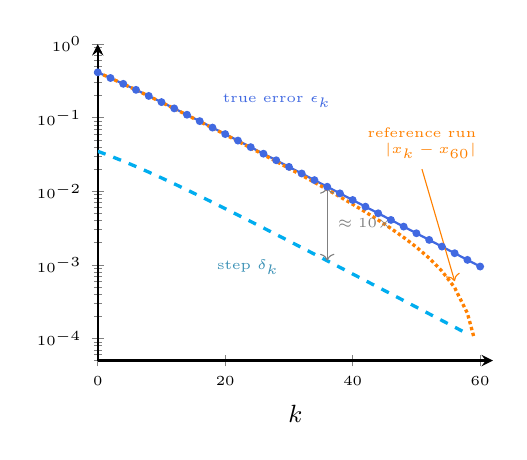
\begin{tikzpicture}
\begin{axis}[width=6.6cm, height=5.6cm, ymode=log, axis lines=left,
  xmin=0, xmax=62, ymin=5e-5, ymax=1, xlabel={$k$}, thick,
  tick label style={font=\tiny}, label style={font=\small}]
  \addplot[accent, mark=*, mark size=1pt] coordinates {(0,0.4142) (2,0.3467) (4,0.2888) (6,0.2395) (8,0.1979) (10,0.163) (12,0.1339) (14,0.1098) (16,0.08987) (18,0.07344) (20,0.05994) (22,0.04888) (24,0.03982) (26,0.03242) (28,0.02639) (30,0.02146) (32,0.01745) (34,0.01418) (36,0.01153) (38,0.009366) (40,0.007609) (42,0.00618) (44,0.005019) (46,0.004076) (48,0.00331) (50,0.002688) (52,0.002183) (54,0.001772) (56,0.001439) (58,0.001168) (60,0.0009484)};
  \addplot[orange, densely dotted, very thick] coordinates {(0,0.4133) (2,0.3458) (4,0.2878) (6,0.2385) (8,0.1969) (10,0.1621) (12,0.133) (14,0.1089) (16,0.08892) (18,0.07249) (20,0.05899) (22,0.04793) (24,0.03887) (26,0.03148) (28,0.02544) (30,0.02051) (32,0.0165) (34,0.01324) (36,0.01058) (38,0.008418) (40,0.00666) (42,0.005232) (44,0.004071) (46,0.003128) (48,0.002362) (50,0.00174) (52,0.001234) (54,0.0008237) (56,0.0004904) (58,0.0002198) (59,0.0001055)};
  \addplot[cyan, dashed, very thick] coordinates {(0,0.035) (2,0.03011) (4,0.02567) (6,0.0217) (8,0.01822) (10,0.01521) (12,0.01263) (14,0.01045) (16,0.008614) (18,0.007081) (20,0.005808) (22,0.004755) (24,0.003887) (26,0.003173) (28,0.002588) (30,0.002108) (32,0.001717) (34,0.001397) (36,0.001136) (38,0.0009241) (40,0.0007512) (42,0.0006105) (44,0.000496) (46,0.000403) (48,0.0003273) (50,0.0002658) (52,0.0002159) (54,0.0001753) (56,0.0001424) (58,0.0001156)};
  \node[accent, font=\tiny, anchor=south west] at (axis cs:18,0.1) {true error $\epsilon_k$};
  \node[orange, font=\tiny, anchor=south east, align=right] (ref) at (axis cs:61,0.02) {reference run\\$|x_k - x_{60}|$};
  \draw[->, orange, thin] (ref.south) -- (axis cs:56,6e-4);
  \node[cyan!70!black, font=\tiny, anchor=north east] at (axis cs:30,1.6e-3) {step $\delta_k$};
  \draw[<->, gray, thin] (axis cs:36,0.0115) -- (axis cs:36,0.00114);
  \node[gray, font=\tiny, right] at (axis cs:36,0.0036) {$\approx 10\times$};
\end{axis}
\end{tikzpicture}\\
\scriptsize $x_{k+1} = x_k - 0.035\,(x_k^2 - 2)$, which converges slowly ($C \approx 0.9$) to $\sqrt 2$
\end{column}
\end{columns}
\end{frame}

% ============================================================
\section{Summary}
% ============================================================

\begin{frame}{Summary}
\begin{columns}[T]
\begin{column}{0.48\textwidth}
\begin{block}{Growth and limits}
\footnotesize
\begin{itemize}
  \item $n^a$: straight on \texttt{loglog} (slope $a$); $b^n$: straight on \texttt{semilogy} (slope $\log b$). Split test to pick the model.
  \item $x_k \to x_\ast$: after some $K$, all terms stay within any tolerance of $x_\ast$.
  \item Limits of $x_{k+1} = g(x_k)$ are fixed points $x_\ast = g(x_\ast)$; attracting if $|g'(x_\ast)| < 1$. Cobweb plots show it.
\end{itemize}
\end{block}
\end{column}
\begin{column}{0.48\textwidth}
\begin{block}{Order of convergence}
\footnotesize
\begin{itemize}
  \item $\epsilon_{k+1} \approx C\,\epsilon_k^{\,q}$: sublinear (ratio $\to 1$), linear ($q = 1$, $C < 1$), superlinear ($q > 1$), quadratic ($q = 2$, digits double).
  \item \texttt{semilogy} of $\epsilon_k$: flattens / straight / bends down.
  \item Measure $q$: slope of $\log\epsilon_{k+1}$ vs.\ $\log\epsilon_k$, or $q_k$ from three errors; use errors above $\approx 10^{-14}$.
  \item $x_\ast$ unknown: use a reference run or the steps $\delta_k$.
\end{itemize}
\end{block}
\end{column}
\end{columns}
\end{frame}

\end{document}
